
\typeout{************************************************}
\typeout{Chapter 4 Calculus in the 17th and 18th Centuries}
\typeout{************************************************}
%
\begin{chapterptx}{Calculus in the 17th and 18th Centuries}{}{Calculus in the 17th and 18th Centuries}{}{}{x:chapter:CalcIn17th18thCentury}
	%
	%
	\typeout{************************************************}
	\typeout{Section 4.1 Newton and Leibniz Get Started}
	\typeout{************************************************}
	%
	\begin{sectionptx}{Newton and Leibniz Get Started}{}{Newton and Leibniz Get Started}{}{}{x:section:CalcIn17th18thCentury-NewtLeibStart}
		%
		%
		\typeout{************************************************}
		\typeout{Subsection 4.1.1 Leibniz's Calculus Rules}
		\typeout{************************************************}
		%
		\begin{subsectionptx}{Leibniz's Calculus Rules}{}{Leibniz's Calculus Rules}{}{}{x:subsection:sec_leibn-calc-rules}
			\begin{figureptx}{\href{https://mathshistory.st-andrews.ac.uk/Biographies/Leibniz/}{Gottfried Wilhelm Leibniz}\protect\footnotemark{}}{g:figure:idp41}{}%
				\index{Leibniz, Gottfried Wilhelm!portrait of}%
				\begin{image}{0.325}{0.35}{0.325}%
					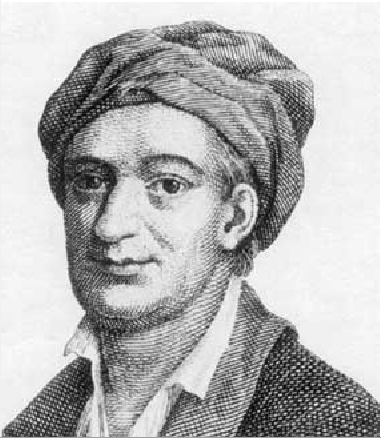
\includegraphics[width=\linewidth]{external/images/Leibniz.png}
				\end{image}%
				\tcblower
			\end{figureptx}%
			\footnotetext[7]{\nolinkurl{mathshistory.st-andrews.ac.uk/Biographies/Leibniz/}\label{g:fn:idp42}}%
			The rules for calculus were first laid out in Gottfried Wilhelm Leibniz's 1684 paper\index{Leibniz, Gottfried Wilhelm!first calculus publication} \textit{Nova methodus pro maximis et minimis, itemque tangentibus, quae nec fractas nec irrationales, quantitates moratur, et singulare pro illi calculi genus} (A New Method for Maxima and Minima as Well as Tangents, Which is Impeded Neither by Fractional Nor by Irrational Quantities, and a Remarkable Type of Calculus for This). Leibniz started with subtraction.  That is, if \(x_1\) and \(x_2\) are very close together then their difference, \(\Delta
			x=x_2-x_1\), is very small.  He expanded this idea to say that if \(x_1\) and \(x_2\) are \emph{infinitely} close together (but still distinct) then their difference, \(\dx{ x}\), is infinitesimally small (but not zero).%
			\begin{aside}{\textit{Calculus Differentialis}.}{g:aside:idp43}%
				This translates, loosely, as the calculus of differences.%
			\end{aside}
			This idea is logically very suspect and Leibniz knew it.  But he also knew that when he used his \textit{calculus differentialis} he was getting correct answers to some very hard problems.  So he persevered.%
			\par
			Leibniz called both \(\Delta x\) and \(\dx{ x}\) ``differentials'' (Latin for difference) because he thought of them as, essentially, the same thing.  Over time it has become customary to refer to the infinitesimal \(\dx{ x}\) as a differential, reserving ``difference'' for the finite case, \(\Delta x\).  This is why calculus is often called ``differential calculus.''%
			\par
			In his paper Leibniz gave rules for dealing with these infinitely small differentials.  Specifically, given a variable quantity \(x\), \(dx\) represented an infinitesimal change in \(x\).  Differentials are related via the slope of the tangent line to a curve.  That is, if \(y=f(x)\), then \(\dx{ y}\) and \(\dx{ x}\) are related by%
			\begin{equation*}
				\dx{ y}=\text{ (slope of the tangent line) } \cdot \dx{ x}\text{.}
			\end{equation*}
			%
			\par
			Leibniz then divided by \(\dx{ x}\) giving%
			\begin{equation*}
				\dfdx{y}{x}= \text{ (slope of the tangent line). }
			\end{equation*}
			%
			\par
			The elegant and expressive notation Leibniz invented was so useful that it has been retained through the years despite some profound changes in the underlying concepts.  For example, Leibniz and his contemporaries would have viewed the symbol \(\dfdx{y}{x}\) as an actual quotient of infinitesimals, whereas today we define it via the limit concept first suggested by Newton.  \index{Newton, Isaac}%
			\par
			As a result the rules governing these differentials are very modern in appearance: \index{Leibniz, Gottfried Wilhelm!differentiation rules}%
			\begin{align*}
				\dx{(\text{ constant } )}\amp =0\\
				\dx{(z-y+w+x)}\amp =\dx{ z}-\dx{ y}+\dx{ w}+\dx{ x}\\
				\dx{(xv)}\amp =x\dx{ v}+v\dx{ x}\\
				\dx{\left(\frac{v}{y}\right)}\amp =\frac{y\dx{ v}-v\dx{ y}}{yy}\\
				\intertext{and, when \(a\) is an integer:}
				\dx{(x^a)}\amp =ax^{a-1}\dx{ x}\text{.}
			\end{align*}
			%
			\par
			Leibniz states these rules without proof: ``. . . the demonstration of all this will be easy to one who is experienced in such matters . . ..'' As an example, mathematicians in Leibniz's day would be expected to understand intuitively that if \(c\) is a constant, then \(d(c)=c-c=0\).  Likewise, \(d(x+y)=dx+dy\) is really an extension of \((x_2+y_2)-(x_1+y_1)=(x_2-x_1)+(y_2-y_1)\).%
		\end{subsectionptx}
		%
		%
		\typeout{************************************************}
		\typeout{Subsection 4.1.2 Leibniz's Approach to the Product Rule}
		\typeout{************************************************}
		%
		\begin{subsectionptx}{Leibniz's Approach to the Product Rule}{}{Leibniz's Approach to the Product Rule}{}{}{x:subsection:LeibnizProductRule}
			\index{Leibniz, Gottfried Wilhelm} The explanation of the product rule using differentials is a bit more involved, but Leibniz expected that mathematicans would be fluent enough to derive it.  The product \(p=xv\) can be thought of as the area of the following rectangle%
			\begin{figureptx}{}{x:figure:fig1}{}%
				\begin{image}{0.25}{0.5}{0.25}%
					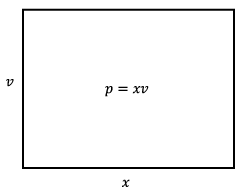
\includegraphics[width=\linewidth]{external/images/fig1.png}
				\end{image}%
				\tcblower
			\end{figureptx}%
			With this in mind, \(\dx{ p}=\dx{(xv)}\) can be thought of as the change in area when \(x\) is changed by \(\dx{ x}\) and \(v\) is changed by \(\dx{ v}\).  This can be seen as the L shaped region in the following drawing.%
			\begin{figureptx}{}{x:figure:fig2}{}%
				\begin{image}{0.05}{0.9}{0.05}%
					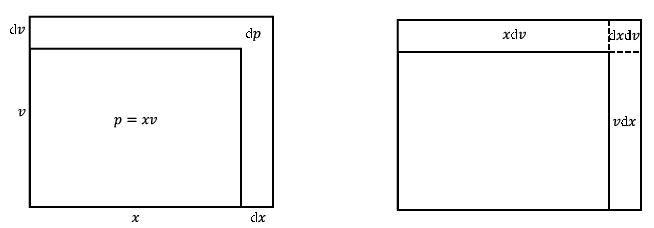
\includegraphics[width=\linewidth]{external/images/fig2.png}
				\end{image}%
				\tcblower
			\end{figureptx}%
			By dividing the L shaped region into 3 rectangles we obtain%
			\begin{equation}
				\dx{(xv)}=x\dx{ v}+v\dx{ x}+\dx{ x}\,\dx{ v}\text{.}\label{x:men:eq_LeibnizProductRule}
			\end{equation}
			%
			\par
			Even though \(\dx{ x}\) and \(\dx{ v}\) are infinitely small, Leibniz reasoned that \(\dx{ x}\,\dx{ v}\) is \emph{even more} infinitely small (quadratically infinitely small?)  compared to \(x\dx{ v}\) and \(v\dx{ x}\) and can thus be ignored leaving%
			\begin{equation*}
				\dx{ (xv)}=x\dx{ v}+v\dx{ x}\text{.}
			\end{equation*}
			%
			\par
			You should feel some discomfort at the idea of simply tossing the product \(\dx{ x}\,\dx{ v}\) aside because it is ``comparatively small.'' This means you have been well trained, and have thoroughly internalized Newton's \index{Newton, Isaac} dictum~\hyperlink{x:biblio:newton45__sir_isaac_two_treat_quadr}{[{\xreffont 10}]}: ``The smallest errors may not, in mathematical matters, be scorned.'' It is logically untenable to toss aside an expression just because it is small.  Even less so should we be willing to ignore an expression on the grounds that it is ``infinitely smaller'' than another quantity which is itself ``infinitely small.''%
			\par
			Newton and Leibniz both knew this as well as we do.  But they also knew that their methods \emph{worked}.  They gave verifiably correct answers to problems which had, heretofore, been completely intractable.  It is the mark of their genius that both men persevered in spite of the very evident difficulties their methods entailed.%
		\end{subsectionptx}
		%
		%
		\typeout{************************************************}
		\typeout{Subsection 4.1.3 Newton's Approach to the Product Rule}
		\typeout{************************************************}
		%
		\begin{subsectionptx}{Newton's Approach to the Product Rule}{}{Newton's Approach to the Product Rule}{}{}{x:subsection:NewtonsApproach}
			In the Principia, Newton ``proved'' the Product Rule as follows: Let \(x\) and \(v\) be ``flowing quantites'' and consider the rectangle, \(R\), whose sides are \(x\) and \(v\).  \(R\) is also a flowing quantity and we wish to find its fluxion (derivative) at any time.%
			\begin{historical}{Newton's `Method of Fluxions'.}{g:historical:idp44}%
				Newton's approach to calculus \textemdash{} his `Method of Fluxions' \textemdash{} depended fundamentally on motion. That is, he viewed his variables (fluents) as changing (flowing or fluxing) in time.  The rate of change of a fluent he called a fluxion.  As a foundation both Leibniz's and Newton's approaches have fallen out of favor, although both are still universally used as a conceptual approach, a ``way of thinking,'' about the ideas of calculus.%
			\end{historical}
			First increment \(x\) and \(v\) by \(\frac{\Delta x}{2}\) and \(\frac{\Delta v}{2}\) respectively. Then the corresponding increment of \(R\) is%
			\begin{equation}
				\left(x+\frac{\Delta x}{2}\right)\left(v+\frac{\Delta v}{2}\right) = xv + x\frac{\Delta v}{2} + v\frac{\Delta x}{2} +\frac{\Delta x\Delta v}{4}\text{.}\label{x:men:eq_prodruleinc}
			\end{equation}
			%
			\par
			Now decrement \(x\) and \(v\) by the same amounts:%
			\begin{equation}
				\left(x-\frac{\Delta x}{2}\right)\left(v-\frac{\Delta v}{2}\right) = xv - x\frac{\Delta v}{2} - v\frac{\Delta x}{2} + \frac{\Delta x\Delta v}{4}\text{.}\label{x:men:eq_prodruledec}
			\end{equation}
			%
			\par
			Subtracting the right side of \hyperref[x:men:eq_prodruledec]{equation~({\xreffont\ref{x:men:eq_prodruledec}})} from the right side of \hyperref[x:men:eq_prodruleinc]{equation~({\xreffont\ref{x:men:eq_prodruleinc}})} gives%
			\begin{equation*}
				\Delta R = x\Delta v + v\Delta x
			\end{equation*}
			which is the total change of \(R = xv\) over the intervals \(\Delta x\) and \(\Delta v\) and also recognizably the Product Rule.%
			\begin{figureptx}{\href{https://mathshistory.st-andrews.ac.uk/Biographies/Newton/}{Isaac Newton}\protect\footnotemark{}}{x:figure:Newton}{}%
				\index{Newton, Isaac!portrait of}%
				\begin{image}{0.325}{0.35}{0.325}%
					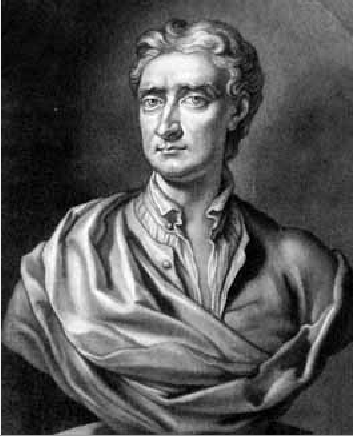
\includegraphics[width=\linewidth]{external/images/Newton.png}
				\end{image}%
				\tcblower
			\end{figureptx}%
			\footnotetext[8]{\nolinkurl{mathshistory.st-andrews.ac.uk/Biographies/Newton/}\label{g:fn:idp45}}%
			This argument is no better than Leibniz's as it relies heavily on the number \(1/2\) to make it work.  If we take any other increments in \(x\) and \(v\) whose total lengths are \(\Delta x\) and \(\Delta v\) it will simply not work.  Try it and see.%
			\par
			In Newton's defense, he wasn't really trying to justify his mathematical methods in the Principia.  His attention there was on physics, not math, so he was really just trying to give a convincing demonstration of his methods.  You may decide for yourself how convincing his demonstration is.%
			\par
			\index{Lagrange, Joseph-Louis} Notice that there is no mention of limits of difference quotients or derivatives.  In fact, the term derivative was not coined until 1797, by Lagrange.  In a sense, these topics were not necessary at the time, as Leibniz and Newton both assumed that the curves they dealt with had tangent lines and, in fact, Leibniz explicitly used the tangent line to relate two differential quantities.  This was consistent with the thinking of the time and for the duration of this chapter we will also assume that all quantities are differentiable.  As we will see later this assumption leads to difficulties.%
			\par
			Both Newton and Leibniz were satisfied that their calculus provided answers that agreed with what was known at the time.  For example \(\dx{ \left(x^2\right)}=\dx{\left(xx\right)}=x\dx{ x}+x\dx{ x}=2x\dx{ x}\) and \(\dx{\left(x^3\right)}=\dx{\left(x^2x\right)}=x^2\dx{ x}+x\dx{\left(x^2\right)}\) \(=x^2+x\left(2x\dx{ x}\right)=3x^2\dx{ x}\),\(\) results that were essentially derived by others in different ways.%
			\begin{problem}{}{g:problem:idp46}%
				\begin{enumerate}[font=\bfseries,label=(\alph*),ref=\alph*]
					\item{}Use Leibniz's product rule \(\dx{ \left(xv\right)}=x\dx{ v}+v\dx{ x}\) to show that if \(n\) is a positive integer then \(\dx{ \left(x^n\right)}=nx^{n-1}\dx{ x}\)%
					\item{}Use Leibniz's product rule to derive the quotient rule%
					\begin{equation*}
						\dx{ \left(\frac{v}{y}\right)}=\frac{y\,\dx{ v}-v\,\dx{ y}}{yy}\text{.}
					\end{equation*}
					%
					\item{}Use the quotient rule to show that if \(n\)is a positive integer, then%
					\begin{equation*}
						\dx{ \left(x^{-n}\right)}=-nx^{-n-1}\dx{ x}.
					\end{equation*}
					%
				\end{enumerate}
			\end{problem}
			\begin{problem}{}{g:problem:idp47}%
				\index{differentiation!power rule with fractional exponents} Let \(p\) and \(q\) be integers with \(q\neq 0\). Show that \(\dx{ \left(x^{\frac{p}{q}}\right)}=\frac{p}{q}x^{\frac{p}{q}-1}\dx{ x}\)%
			\end{problem}
			Leibniz also provided applications of his calculus to prove its worth. As an example he derived Snell's Law of Refraction from his calculus rules as follows.%
			\par
			Given that light travels through air at a speed of \(v_a\) and travels through water at a speed of \(v_w\) the problem is to find the fastest path from point \(A\) to point \(B\).%
			\begin{figureptx}{}{x:figure:snellfig}{}%
				\begin{image}{0.125}{0.75}{0.125}%
					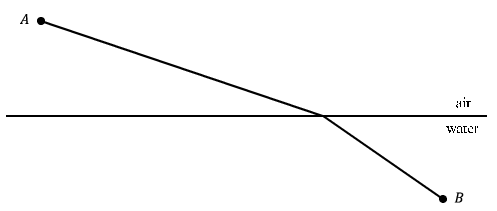
\includegraphics[width=\linewidth]{external/images/snellfig.png}
				\end{image}%
				\tcblower
			\end{figureptx}%
			According to Fermat's Principle of Least Time, this fastest path is the one that light will travel.%
			\par
			Using the fact that \(\text{ Time } =\text{ Distance }
			/\text{ Velocity }\) and the labeling in the picture below we can obtain a formula for the time \(T\) it takes for light to travel from \(A\) to \(B\).%
			\begin{figureptx}{}{x:figure:snellfig2}{}%
				\begin{image}{0.125}{0.75}{0.125}%
					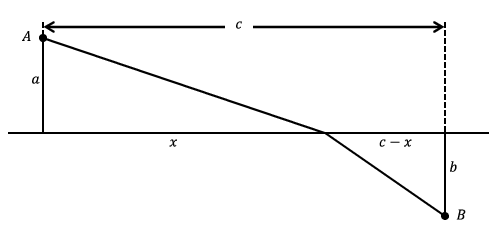
\includegraphics[width=\linewidth]{external/images/snellfig2.png}
				\end{image}%
				\tcblower
			\end{figureptx}%
			%
			\begin{equation*}
				T=\frac{\sqrt{x^2+a^2}}{v_a}+\frac{\sqrt{(c-x)^2+b^2}}{v_w}
			\end{equation*}
			%
			\par
			Using the rules of Leibniz's calculus, we obtain%
			\begin{align*}
				\dx{ T}\amp = \left(\frac{1}{v_a}\frac{1}{2}\left(x^2+a^2\right)^{-\frac{1}{2}} (2x)+\frac{1}{v_w}\frac{1}{2}((c-x)^2+b^2)^{-\frac{1}{2}}(2(c-x)(-1))\right) \dx{ x}\\
				\amp =\left(\frac{1}{v_a}\frac{x}{\sqrt{x^2+a^2}}-\frac{1}{v_w}\frac{c-x}{\sqrt{(c-x)^2+b^2}}\right)\dx{ x}\text{.}
			\end{align*}
			%
			\par
			Using the fact that at the minimum value for \(T\), \(\dx{ T}=0\), we have that the fastest path from \(A\)to \(B\) must satisfy \(\frac{1}{v_a}\frac{x}{\sqrt{x^2+a^2}}=\frac{1}{v_w}\frac{c-x}{\sqrt{(c-x)^2+b^2}}\). Inserting the following angles%
			\begin{figureptx}{}{x:figure:snellfig3}{}%
				\begin{image}{0.125}{0.75}{0.125}%
					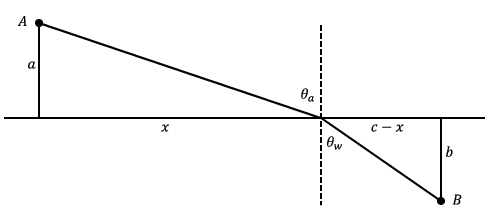
\includegraphics[width=\linewidth]{external/images/snellfig3.png}
				\end{image}%
				\tcblower
			\end{figureptx}%
			we get that the path that light travels must satisfy \(\frac{\sin\theta_a}{v_a}=\frac{\sin\theta_w}{v_w}\) which is Snell's Law.%
			\par
			\index{Bernoulli, Johann}\index{Brachistochrone problem, the} To compare 18th century and modern techniques we will consider Johann Bernoulli's solution of the Brachistochrone problem. In 1696, Bernoulli posed, and solved, the Brachistochrone problem; that is, to find the shape of a frictionless wire joining points A and B so that the time it takes for a bead to slide down under the force of gravity is as small as possible.%
			\begin{figureptx}{}{x:figure:brachfig1}{}%
				\begin{image}{0.125}{0.75}{0.125}%
					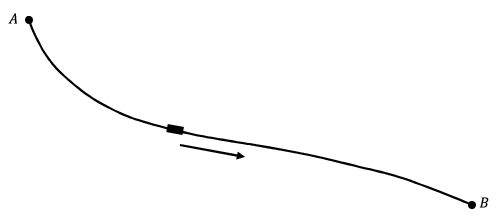
\includegraphics[width=\linewidth]{external/images/brachfig1.png}
				\end{image}%
				\tcblower
			\end{figureptx}%
			Bernoulli posed this ``path of fastest descent'' problem to challenge the mathematicians of Europe and used his solution to demonstrate the power of Leibniz's calculus as well as his own ingenuity.  \index{Bernoulli, Johann!Bernoulli's challenge}%
			\begin{quote}%
				I, Johann Bernoulli, address the most brilliant mathematicians in the world. Nothing is more attractive to intelligent people than an honest, challenging problem, whose possible solution will bestow fame and remain as a lasting monument. Following the example set by Pascal, Fermat, etc., I hope to gain the gratitude of the whole scientific community by placing before the finest mathematicians of our time a problem which will test their methods and the strength of their intellect. If someone communicates to me the solution of the proposed problem, I shall publicly declare him worthy of praise. \hyperlink{x:biblio:Bernoulli_bio_mactutor}{[{\xreffont 11}]}%
			\end{quote}
			\begin{figureptx}{\href{https://mathshistory.st-andrews.ac.uk/Biographies/Bernoulli_Johann/}{Johann Bernoulli}\protect\footnotemark{}}{g:figure:idp48}{}%
				\index{Bernoulli, Johann!portrait of}%
				\begin{image}{0.325}{0.35}{0.325}%
					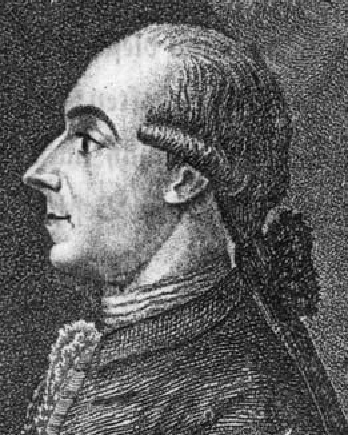
\includegraphics[width=\linewidth]{external/images/BernoulliJohann.png}
				\end{image}%
				\tcblower
			\end{figureptx}%
			\footnotetext[9]{\nolinkurl{mathshistory.st-andrews.ac.uk/Biographies/Bernoulli_Johann/}\label{g:fn:idp49}}%
			In addition to Johann's, solutions were obtained from Newton, \index{Newton, Isaac} Leibniz, Johann's brother Jacob Bernoulli, \index{Bernoulli Jacob} and the Marquis de l'Hopital \hyperlink{x:biblio:struik69__sourc_book_mathem}{[{\xreffont 15}]}.  At the time there was an ongoing and very vitriolic controversy raging over whether Newton or Leibniz had been the first to invent calculus.  An advocate of the methods of Leibniz, Bernoulli did not believe Newton would be able to solve the problem using his methods. Bernoulli attempted to embarrass Newton by sending him the problem.  However Newton did solve it.%
			\par
			At this point in his life Newton had all but quit science and mathematics and was fully focused on his administrative duties as Master of the Mint.  In part due to rampant counterfeiting, England's money had become severely devalued and the nation was on the verge of economic collapse.  The solution was to recall all of the existing coins, melt them down, and strike new ones.  As Master of the Mint this job fell to Newton \hyperlink{x:biblio:levenson09__newton_count}{[{\xreffont 8}]}.  As you might imagine this was a rather Herculean task.  Nevertheless, according to his niece:%
			\begin{quote}%
				When the problem in 1696 was sent by Bernoulli\textendash{}Sir I.N. was in the midst of the hurry of the great recoinage and did not come home till four from the Tower very much tired, but did not sleep till he had solved it, which was by four in the morning.%
			\end{quote}
			He is later reported to have complained, ``I do not love . . . to be . . . teezed by forreigners about Mathematical things'' \hyperlink{x:biblio:dunham90__journ_throug_genius}{[{\xreffont 2}]}.%
			\par
			\index{Bernoulli, Johann!\textit{"Tanquam ex ungue leonem"}} Newton submitted his solution anonymously, presumably to avoid more controversy.  Nevertheless the methods used were so distinctively Newton's that Bernoulli is said to have exclaimed ``\textit{Tanquam ex ungue leonem}.''%
			\begin{aside}{\textit{Tanquam ex ungue leonem}.}{g:aside:idp50}%
				``I know the lion by his claw.''%
			\end{aside}
			\index{Brachistochrone problem, the!Bernoulli's solution} Bernoulli's ingenious solution starts, interestingly enough, with Snell's Law of Refraction. He begins by considering the stratified medium in the following figure, where an object travels with velocities \(v_1,\,v_2,\,v_3,\,\ldots\) in the various layers.%
			\begin{figureptx}{}{x:figure:brachfig2}{}%
				\begin{image}{0.125}{0.75}{0.125}%
					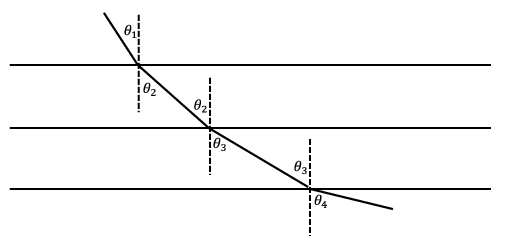
\includegraphics[width=\linewidth]{external/images/brachfig2.png}
				\end{image}%
				\tcblower
			\end{figureptx}%
			By repeatedly applying Snell's Law he concluded that the fastest path must satisfy%
			\begin{equation*}
				\frac{\sin \theta_1}{v_1}=\frac{\sin \theta_2}{v_2}=\frac{\sin\theta_3}{v_3}=\cdots\text{.}
			\end{equation*}
			%
			\par
			In other words, the ratio of the sine of the angle that the curve makes with the vertical and the speed remains constant along this fastest path.%
			\par
			If we think of a continuously changing medium as stratified into infinitesimal layers and extend Snell's law to an object whose speed is constantly changing,%
			\begin{figureptx}{}{x:figure:snellfig4}{}%
				\begin{image}{0.125}{0.75}{0.125}%
					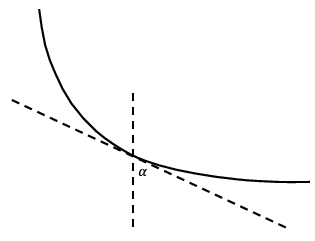
\includegraphics[width=\linewidth]{external/images/snellfig4.png}
				\end{image}%
				\tcblower
			\end{figureptx}%
			then along the fastest path, the ratio of the sine of the angle that the curve's tangent makes with the vertical, \(\alpha\), and the speed, \(v\), must remain constant.%
			\begin{equation*}
				\frac{\text{ sin } \alpha}{v}=c\text{.}
			\end{equation*}
			%
			\par
			If we include axes and let \(P\) denote the position of the bead at a particular time then we have the following picture.%
			\begin{figureptx}{}{x:figure:snellfig5}{}%
				\begin{image}{0.125}{0.75}{0.125}%
					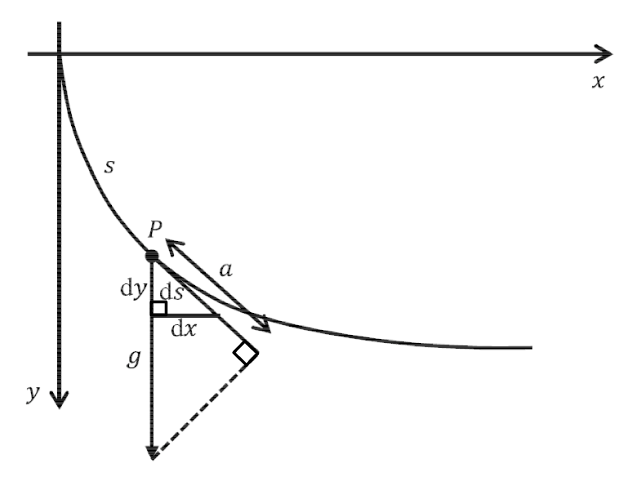
\includegraphics[width=\linewidth]{external/images/snellfig5.png}
				\end{image}%
				\tcblower
			\end{figureptx}%
			In the above figure, \(s\) denotes the length that the bead has traveled down to point \(P\)(that is, the arc length of the curve from the origin to that point) and \(a\) denotes the tangential component of the acceleration due to gravity \(g\).  Since the bead travels only under the influence of gravity then \(\dfdx{v}{t}=a\).%
			\par
			To get a sense of how physical problems were approached using Leibniz's calculus we will use the above equation to show that \(v=\sqrt{2gy}\).%
			\par
			By similar triangles we have \(\frac{a}{g}=\frac{\dx{ y}}{\dx{ s}}\). As a student of Leibniz, Bernoulli would have regarded \(\frac{\dx{ y}}{\dx{ s}}\) as a fraction so%
			\begin{align*}
				a\dx{ s} \amp = g\dx{ y}\\
				\intertext{and since acceleration is the rate of change of velocity we have}
				\frac{\dx{ v}}{\dx{ t}}\dx{ s} \amp = g\dx{ y}.\\
				\intertext{Again, 18th century European mathematicians regarded \(\dx{ v}, \dx{ t}\), and \(\dx{ s}\) as infinitesimally small numbers which nevertheless obey all of the usual rules of algebra. Thus we can rearrange the above to get}
				\frac{\dx{ s}}{\dx{ t}}\dx{ v} \amp = g\dx{ y}.\\
				\intertext{Since \(\frac{\dx{ s}}{\dx{ t}}\) is the rate of change of position with respect to time it is, in fact, the velocity of the bead. That is}
				v\dx{ v} \amp = g\dx{ y}.\\
				\intertext{Bernoulli would have interpreted this as a statement that two rectangles of height \(v\) and \(g\), with respective widths \(\dx{ v}\) and \(\dx{ y}\) have equal area. Summing (integrating) all such rectangles we get:}
				\int{}v\dx{ v} \amp = \int{}g\dx{ y}\\
				\frac{v^2}{2} \amp = gy
			\end{align*}
			or%
			\begin{equation}
				v=\sqrt{2gy}\text{.}\label{x:men:eq_brach_vel}
			\end{equation}
			%
			\par
			You are undoubtedly uncomfortable with the cavalier manipulation of infinitesimal quantities you've just witnessed, so we'll pause for a moment now to compare a modern development of \hyperref[x:men:eq_brach_vel]{equation~({\xreffont\ref{x:men:eq_brach_vel}})} to Bernoulli's. As before we begin with the equation:%
			\begin{align*}
				\frac{a}{g}\amp = \dfdx{y}{s}\\
				a \amp = g\dfdx{y}{s}.\\
				\intertext{Moreover, since acceleration is the derivative of velocity this is the same as:}
				\dfdx{v}{t} \amp = g\dfdx{y}{s}.\\
				\intertext{Now observe that by the Chain Rule \(\dfdx{v}{t} = \dfdx{v}{s}\dfdx{s}{t}\). The physical interpretation of this formula is that velocity will depend on \(s\), how far down the wire the bead has moved, but that the distance traveled will depend on how much time has elapsed. Therefore}
				\dfdx{v}{s}\dfdx{s}{t} \amp = g\dfdx{y}{s}\\
				\intertext{or}
				\dfdx{s}{t}\dfdx{v}{s} \amp = g\dfdx{y}{s}\\
				\intertext{and since \(\dfdx{s}{t} = v\) we have}
				v\dfdx{v}{s} \amp = g\dfdx{y}{s}\\
				\intertext{Integrating both sides with respect to \(s\) gives:}
				\int{}v\dfdx{v}{s}d s \amp = g\int{}\dfdx{y}{s}d s\\
				\int{}vd v \amp = g\int{}d y\\
				\intertext{and integrating gives}
				\frac{v^2}{2} \amp = gy
			\end{align*}
			as before.%
			\par
			In effect, in the modern formulation we have traded the simplicity and elegance of differentials for a comparatively cumbersome repeated use of the Chain Rule. No doubt you noticed when taking Calculus that in the differential notation of Leibniz,\index{Leibniz, Gottfried Wilhelm} the Chain Rule looks like ``canceling'' an expression in the top and bottom of a fraction: \(\dfdx{y}{u}\dfdx{u}{x} = \dfdx{y}{x}\). This is because for 18th century mathematicians, this is exactly what it was.%
			\par
			To put it another way, 18th century mathematicians wouldn't have recognized a need for what we call the Chain Rule because this operation was a triviality for them. Just reduce the fraction. This begs the question: Why did we abandon such a clear, simple interpretation of our symbols in favor of the, comparatively, more cumbersome modern interpretation? This is one of the questions we will try to answer in this course.%
			\par
			Returning to the Brachistochrone problem we observe that%
			\begin{align}
				\frac{\sin\alpha}{v} \amp = c\notag\\
				\intertext{and since \(\sin\alpha = \frac{d x}{d s}\)   we see that}
				\frac{\frac{d x}{d s}}{\sqrt{2gy}} \amp = c\notag\\
				\frac{d x}{\sqrt{2gy(ds)^2}} \amp = c\notag\\
				\frac{d x}{\sqrt{2gy\left[(d x)^2+(d y)^2\right]}} \amp = c\text{.}\label{x:mrow:eq_Brachistochrone}
			\end{align}
			%
			\par
			Bernoulli was then able to solve this differential equation.%
			\begin{problem}{}{g:problem:idp51}%
				\index{Brachistochrone problem, the} Show that the equations \(x=\frac{\phi-\sin \phi}{4gc^2},\,y=\frac{1-\cos \phi}{4gc^2}\) satisfy equation \hyperref[x:mrow:eq_Brachistochrone]{({\xreffont\ref{x:mrow:eq_Brachistochrone}})}. Bernoulli recognized this solution to be an inverted cycloid, the curve traced by a fixed point on a circle as the circle rolls along a horizontal surface.%
			\end{problem}
			This illustrates the state of calculus in the late 1600's and early 1700's; the foundations of the subject were a bit shaky but there was no denying its power.%
		\end{subsectionptx}
	\end{sectionptx}
	%
	%
	\typeout{************************************************}
	\typeout{Section 4.2 Power Series as Infinite Polynomials}
	\typeout{************************************************}
	%
	\begin{sectionptx}{Power Series as Infinite Polynomials}{}{Power Series as Infinite Polynomials}{}{}{x:section:ExponentAdditionProperty}
		\index{polynomials!infinite} Applied to polynomials, the rules of differential and integral calculus are straightforward.  Indeed, differentiating and integrating polynomials represent some of the easiest tasks in a calculus course.  For example, computing \(\int(7-x+x^2)\dx{ x}\) is relatively easy compared to computing \(\int\sqrt[3]{1+x^3}\dx{ x}\).  Unfortunately, not all functions can be expressed as a polynomial.  For example, \(f(x)=\sin x\) cannot be since a polynomial has only finitely many roots and the sine function has infinitely many roots, namely \(\{n\pi|\,n\in\ZZ\}\).  A standard technique in the 18th century was to write such functions as an ``infinite polynomial,'' what we typically refer to as a power series.  Unfortunately an ``infinite polynomial'' is a much more subtle object than a mere polynomial, which by definition is finite. For now we will not concern ourselves with these subtleties.  We will follow the example of our forebears and manipulate all ``polynomial-like'' objects (finite or infinite) as if they are polynomials.%
		\begin{definition}{}{x:definition:def_PowerSeries}%
			\index{power series!definition of} A \terminology{power series centered at \(\boldsymbol{a}\)} is a series of the form%
			\begin{equation*}
				\sum_{n=0}^\infty a_n(x-a)^n=a_0+a_1(x-a)+a_2(x-a)^2+\cdots\text{.}
			\end{equation*}
			%
			\par
			Often we will focus on the behavior of power series \(\sum_{n=0}^\infty a_nx^n\), centered around \(0\), as the series centered around other values of \(a\) are obtained by shifting a series centered at \(0\).%
		\end{definition}
		Before we continue, we will make the following notational comment. The most advantageous way to represent a series is using summation notation since there can be no doubt about the pattern to the terms. After all, this notation contains a formula for the general term. This being said, there are instances where writing this formula is not practical. In these cases, it is acceptable to write the sum by supplying the first few terms and using ellipses (the three dots). If this is done, then enough terms must be included to make the pattern clear to the reader.%
		\par
		Returning to our definition of a power series, consider, for example, the \index{series!Geometric series!naive derivation} geometric series \(\sum_{n=0}^\infty x^n=1+x+x^2+\cdots\). If we multiply this series by \((1-x)\), we obtain%
		\begin{equation*}
			(1-x)(1+x+x^2+\cdots)=(1+x+x^2+\cdots)-(x+x^2+x^3+\cdots)=1\text{.}
		\end{equation*}
		%
		\par
		This leads us to the power series representation%
		\begin{equation*}
			\frac{1}{1-x}=1+x+x^2+\cdots=\sum_{n=0}^\infty x^n\text{.}
		\end{equation*}
		%
		\par
		If we substitute \(x=\frac{1}{10}\) into the above, we obtain%
		\begin{equation*}
			1+\frac{1}{10}+\left(\frac{1}{10}\right)^2+\left(\frac{1}{10}\right)^3+ \cdots=\frac{1}{1-\frac{1}{10}}=\frac{10}{9}\text{.}
		\end{equation*}
		%
		\par
		This agrees with the fact that \(.333\ldots=\frac{1}{3}\), and so \(.111\ldots=\frac{1}{9}\), and \(1.111\ldots=\frac{10}{9}\).%
		\par
		There are limitations to these formal manipulations however. Substituting \(x=1\) or \(x=2\) yields the questionable results%
		\begin{equation*}
			\frac{1}{0}=1+1+1+\cdots\,\text{  and  }  \,\frac{1}{-1}=1+2+2^2+\cdots\text{.}
		\end{equation*}
		%
		\par
		We are missing something important here, though it may not be clear exactly what. A series representation of a function works \emph{sometimes,} but there are some problems. For now, we will continue to follow the example of our 18th century predecessors and ignore them. That is, for the rest of this section we will focus on the formal manipulations to obtain and use power series representations of various functions. Keep in mind that this is all highly suspect until we can resolve problems like those just given.%
		\par
		Power series became an important tool in analysis in the 1700's.  By representing various functions as power series they could be dealt with as if they were (infinite) polynomials.  The following is an example.%
		\begin{example}{}{g:example:idp52}%
			Solve the following Initial Value problem: Find \(y(x)\) given that \(\frac{\dx{ y}}{\dx{ x}}=y,\,y(0)=1\).%
			\begin{aside}{}{g:aside:idp53}%
				A few seconds of thought should convince you that the solution of this problem is \(y(x) = e^x\).  We will ignore this for now in favor of emphasising the technique.%
			\end{aside}
			Assuming the solution can be expressed as a power series we have%
			\begin{equation*}
				y=\sum_{n=0}^\infty a_nx^n=a_0+a_1x+a_2x^2+\cdots\text{.}
			\end{equation*}
			%
			\par
			Differentiating gives us%
			\begin{equation*}
				\frac{\dx{ y}}{\dx{ x}}=a_1+2a_2x+3a_3x^2+4a_4x^3+\ldots\text{.}
			\end{equation*}
			%
			\par
			Since \(\frac{\dx{ y}}{\dx{ x}}=y\) we see that%
			\begin{equation*}
				a_1=a_0\,,\,2a_2=a_1\,,\,3a_3=a_2\,,\,\ldots,\,na_n=a_{n-1}\,,\ldots\text{.}
			\end{equation*}
			%
			\par
			This leads to the relationship%
			\begin{equation*}
				a_n=\frac{1}{n}a_{n-1}=\frac{1}{n(n-1)}a_{n-2}=\cdots=\frac{1}{n!}a_0\text{.}
			\end{equation*}
			%
			\par
			Thus the series solution of the differential equation is%
			\begin{equation*}
				y=\sum_{n=0}^\infty\frac{a_0}{n!}x^n=a_0\sum_{n=0}^\infty\frac{1}{n!}x^n\text{.}
			\end{equation*}
			%
			\par
			Using the initial condition \(y(0)=1\), we get \(1=a_0(1+0+\frac{1}{2!}0^2+\cdots)=a_0\). Thus the solution to the initial problem is \(y=\sum_{n=0}^\infty\frac{1}{n!}x^n\). Let's call this function \(E(x)\). Then by definition%
			\begin{equation*}
				E(x)=\sum_{n=0}^\infty\frac{1}{n!}x^n=1+\frac{x^1}{1!}+\frac{x^2}{2!}+\frac{x^3}{3!}+\,\ldots\text{.}
			\end{equation*}
			%
		\end{example}
		Let's examine some properties of this function. The first property is clear from the definition.%
		\par
		\index{\(e^x\)!\(E(0)=1\)} \terminology{Property 1}. \(E(0)=1\)%
		\par
		\index{\(e^x\)!\(E(x+y)=E(x)E(y)\)} \terminology{Property 2}. \(E(x+y)=E(x)E(y)\).%
		\par
		To see this we multiply the two series together, so we have%
		\begin{align*}
			E(x)E(y) \amp =\left(\sum_{n=0}^\infty\frac{1}{n!}x^n\right)\left(\sum_{n=0}^\infty\frac{1}{n!}y^n\right)\\
			\amp =\left(\frac{x^0}{0!}+\frac{x^1}{1!}+\frac{x^2}{2!}+\frac{x^3}{3!}+\,\ldots\right)\left(\frac{y^0}{0!}+\frac{y^1}{1!}+\frac{y^2}{2!}+\frac{y^3}{3!}+\,\ldots\right)\\
			\amp =\frac{x^0}{0!}\frac{y^0}{0!}+\frac{x^0}{0!}\frac{y^1}{1!}+\frac{x^1}{1!}\frac{y^0}{0!}+\frac{x^0}{0!}\frac{y^2}{2!}+\frac{x^1}{1!}\frac{y^1}{1!}+\frac{x^2}{2!}\frac{y^0}{0!}\\
			\amp \ \ \ \ \ \  +\frac{x^0}{0!}\frac{y^3}{3!}+\frac{x^1}{1!}\frac{y^2}{2!}+\frac{x^2}{2!}\frac{y^1}{1!}+\frac{x^3}{3!}\frac{y^0}{0!}+\,\ldots\\
			\amp =\frac{x^0}{0!}\frac{y^0}{0!}+\left(\frac{x^0}{0!}\frac{y^1}{1!}+ \frac{x^1}{1!}\frac{y^0}{0!}\right)\\
			\amp \ \ \ \ \ \  +\left(\frac{x^0}{0!}\frac{y^2}{2!}+\frac{x^1}{1!}\frac{y^1}{1!}+\frac{x^2}{2!}\frac{y^0}{0!}\right)\\
			\amp \ \ \ \ \ \ +\left(\frac{x^0}{0!}\frac{y^3}{3!}+\frac{x^1}{1!}\frac{y^2}{2!}+\frac{x^2}{2!}\frac{y^1}{1!}+\frac{x^3}{3!}\frac{y^0}{0!}\right)+\,\ldots\\
			\amp =\frac{1}{0!}+\frac{1}{1!}\left(\frac{1!}{0!1!}x^0y^1+\frac{1!}{1!0!}x^1y^0\right)\\
			\amp \ \ \ \ \ \ +\frac{1}{2!}\left(\frac{2!}{0!2!}x^0y^2+\frac{2!}{1!1!}x^1y^1+\frac{2!}{2!0!}x^2y^0\right)\\
			\amp \ \ \ \ \ \ +\frac{1}{3!}\left(\frac{3!}{0!3!}x^0y^3+\frac{3!}{1!2!}x^1y^2+\frac{3!}{2!1!}x^2y^1+\frac{3!}{3!0!}x^3y^0\right)+\ldots
		\end{align*}
		%
		\begin{align}
			E(x)E(y) \amp =\frac{1}{0!}+\frac{1}{1!}\left(\binom{1}{0}x^0y^1+\binom{1}{1}x^1y^0\right)\notag\\
			\amp \ \ \ \ \ \ +\frac{1}{2!}\left(\binom{2}{0}x^0y^2+\binom{2}{1}x^1y^1+\binom{2}{2}x^2y^0\right)\notag\\
			\amp \ \ \ \ \ \ +\frac{1}{3!}\left(\binom{3}{0}x^0y^3+\binom{3}{1}x^1y^2+\binom{3}{2}x^2y^1+\binom{3}{3}x^3y^0\right)+\ldots\notag\\
			\amp =\frac{1}{0!}+\frac{1}{1!}\left(x+y\right)^1+\frac{1}{2!}\left(x+y\right)^2+\frac{1}{3!}\left(x+y\right)^3+\ldots\notag\\
			\amp =E(x+y)\text{.}\label{x:mrow:eq_ExponentAdditionProperty}
		\end{align}
		%
		\par
		\index{\(e^x\)!\(E(m)=\left(E(1)\right)^mE(0)=1\)} \terminology{Property 3}. If \(m\) is a positive integer then \(E(mx)=\left(E(x\right))^m\). In particular, \(E(m)=\left(E(1)\right)^m\).%
		\begin{problem}{}{g:problem:idp54}%
			\index{\(e^x\)!\(E(mx)=\left(E(x\right))^m\)} Prove Property 3.%
		\end{problem}
		\terminology{Property 4}. \(E(-x)=\frac{1}{E(x)}=\left(E(x)\right)^{-1}\).%
		\begin{problem}{}{g:problem:idp55}%
			\index{\(e^x\)!\(E(-x)=\left(E(x)\right)^{-1}\)} Prove Property 4.%
		\end{problem}
		\terminology{Property 5}. If \(n\) is an integer with \(n\neq 0\), then \(E(\frac{1}{n})=\sqrt[n]{E(1)}=\left(E(1)\right)^{1/n}\).%
		\begin{problem}{}{g:problem:idp56}%
			\index{\(e^x\)!\(E(\frac{1}{n})=\left(E(1)\right)^{1/n}\)} Prove Property 5.%
		\end{problem}
		\terminology{Property 6}. If \(m\) and \(n\) are integers with \(n\neq 0\), then \(E\left(\frac{m}{n}\right)=\left(E(1)\right)^{m/n}\).%
		\begin{problem}{}{g:problem:idp57}%
			\index{\(e^x\)!\(E\left(\frac{m}{n}\right)=\left(E(1)\right)^{m/n}\)} Prove Property 6.%
		\end{problem}
		\begin{definition}{}{x:definition:def_e}%
			\index{\(e^x\)!definition of \(e\)} Let \(E(1)\) be denoted by the number \(e\). Using the series \(e=E(1)=\sum_{n=0}^\infty\frac{1}{n!}\), we can approximate \(e\) to any degree of accuracy. In particular \(e\approx 2.71828\).%
		\end{definition}
		In light of Property~6, we see that for any rational number \(r\), \(E(r)=e^r\). Not only does this give us the series representation \(e^r=\sum_{n=0}^\infty\frac{1}{n!}r^n\) for any rational number \(r\), but it gives us a way to define \(e^x\) for irrational values of \(x\) as well. That is, we can define%
		\begin{equation*}
			e^x=E(x)=\sum_{n=0}^\infty\frac{1}{n!}x^n
		\end{equation*}
		for any real number \(x\).%
		\par
		As an illustration, we now have \(e^{\sqrt{2}}=\sum_{n=0}^\infty\frac{1}{n!}\left(\sqrt{2}\right)^n\). The expression \(e^{\sqrt{2}}\) is meaningless if we try to interpret it as one irrational number raised to another. What does it mean to raise anything to the \(\sqrt{2}\) power? However the series \(\sum_{n=0}^\infty\frac{1}{n!}\left(\sqrt{2}\right)^n\) does seem to have meaning and it can be used to extend the exponential function to irrational exponents. In fact, defining the exponential function via this series answers the question we raised in  \hyperref[x:chapter:NumbersRealRational]{Chapter~{\xreffont\ref{x:chapter:NumbersRealRational}}}: What does \(4^{\sqrt{2}}\) mean?%
		\par
		It means \(\displaystyle 4^{\sqrt{2}} = e^{\sqrt{2}\log 4} = \sum_{n=0}^\infty\frac{(\sqrt{2}\log 4)^n}{n!}\).%
		\par
		This may seem to be the long way around just to define something as simple as exponentiation. But this is a fundamentally misguided attitude. Exponentiation only \emph{seems} simple because we've always thought of it as repeated multiplication (in \(\ZZ\)) or root-taking (in \(\QQ\)). When we expand the operation to the real numbers this simply can't be the way we interpret something like \(4^{\sqrt{2}}\). How do you take the product of \(\sqrt{2}\) copies of \(4?\) The concept is meaningless. What we need is an interpretation of \(4^{\sqrt{2}}\) which is consistent with, say \(4^{3/2} = \left(\sqrt{4}\right)^3=8\). This is exactly what the series representation of \(e^x\) provides.%
		\par
		We also have a means of computing integrals as series. For example, the famous ``bell shaped'' curve given by the function \(f(x)=\frac{1}{\sqrt{2\pi}}e^{-\frac{x^2}{2}}\) is of vital importance in statistics and must be integrated to calculate probabilities. The power series we developed gives us a method of integrating this function. For example, we have%
		\begin{align*}
			\int_{x=0}^b\frac{1}{\sqrt{2\pi}}e^{-\frac{x^2}{2}}d x \amp  =\frac{1}{\sqrt{2\pi}}\int_{x=0}^b\left(\sum_{n=0}^\infty\frac{1}{n!}\left(\frac{-x^2}{2}\right)^n\right)d x\\
			\amp =\frac{1}{\sqrt{2\pi}}\,\sum_{n=0}^\infty\left(\frac{\left(-1\right)^n}{n!2^n}\int_{x=0}^bx^{2n}d x\right)\\
			\amp =\frac{1}{\sqrt{2\pi}}\,\sum_{n=0}^\infty\left(\frac{\left(-1\right)^nb^{2n+1}}{n!2^n\left(2n+1\right)}\right)\text{.}
		\end{align*}
		%
		\par
		This series can be used to approximate the integral to any degree of accuracy. The ability to provide such calculations made power series of paramount importance in the 1700's.%
		\begin{problem}{}{g:problem:idp58}%
			\begin{enumerate}[font=\bfseries,label=(\alph*),ref=\alph*]
				\item{}Show that if \(y=\sum_{n=0}^\infty a_nx^n\) satisfies the differential equation \(\frac{\dx^2y}{\dx{ x}^2}=-y\), then%
				\begin{equation*}
					a_{n+2}=\frac{-1}{\left(n+2\right)\left(n+1\right)}\,a_n
				\end{equation*}
				and conclude that%
				\begin{equation*}
					y=a_0+a_1x-\frac{1}{2!}\,a_0x^2-\frac{1}{3!}\,a_1x^3+\frac{1}{4!}\,a_0x^4+\frac{1}{5!}\,a_1x^5-\frac{1}{6!}\,a_0x^6-\frac{1}{7!}\,a_1x^7+\cdots\text{.}
				\end{equation*}
				%
				\item{}Since \(y=\sin x\) satisfies \(\frac{\dx^2y}{\dx{
						x}^2}=-y\), we see that%
				\begin{equation*}
					\sin x=a_0+a_1x-\frac{1}{2!}\,a_0x^2-\frac{1}{3!}\,a_1x^3+\frac{1}{4!}\,a_0x^4+\frac{1}{5!}\,a_1x^5-\frac{1}{6!}\,a_0x^6-\frac{1}{7!}\,a_1x^7+\cdots
				\end{equation*}
				for some constants \(a_0\) and \(a_1\).  Show that in this case \(a_0=0\) and \(a_1=1\) and obtain%
				\begin{equation*}
					\sin x=x-\frac{1}{3!}\,x^3+\frac{1}{5!}x^5-\frac{1}{7!}x^7+\cdots=\sum_{n=0}^\infty\frac{\left(-1\right)^n}{\left(2n+1\right)!}x^{2n+1}\text{.}
				\end{equation*}
				%
			\end{enumerate}
		\end{problem}
		\begin{problem}{}{g:problem:idp59}%
			\begin{enumerate}[font=\bfseries,label=(\alph*),ref=\alph*]
				\item{}Use the series%
				\begin{equation*}
					\sin x=x-\frac{1}{3!}\,x^3+\frac{1}{5!}x^5-\frac{1}{7!}x^7+\cdots=\sum_{n=0}^\infty\frac{\left(-1\right)^n}{\left(2n+1\right)!}x^{2n+1}
				\end{equation*}
				to obtain the series%
				\begin{equation*}
					\cos x=1-\frac{1}{2!}\,x^2+\frac{1}{4!}x^4-\frac{1}{6!}x^6+\cdots=\sum_{n=0}^\infty\frac{\left(-1\right)^n}{\left(2n\right)!}x^{2n}\text{.}
				\end{equation*}
				%
				\item{}Let \(s(x,N)=\sum_{n=0}^N\frac{\left(-1\right)^n}{\left(2n+1\right)!}x^{2n+1}\) and \(c(x,N)=\sum_{n=0}^N\frac{\left(-1\right)^n}{\left(2n\right)!}x^{2n}\) and use a computer algebra system to plot these for\(\,-4\pi\leq x\leq 4\pi,\,\,N=1,2,5,\,10,\,15\). Describe what is happening to the series as N becomes larger.%
			\end{enumerate}
		\end{problem}
		\begin{problem}{}{x:problem:prob_alternating_harmonic_series}%
			Use the geometric series, \(\frac{1}{1-x}=1+x+x^2+x^3+\cdots=\sum_{n=0}^\infty x^n\), to obtain a series for \(\frac{1}{1+x^2}\) and use this to obtain the series%
			\begin{equation*}
				\arctan x=x-\frac{1}{3}x^3+\frac{1}{5}x^5-\cdots=\sum_{n=0}^\infty(-1)^n \frac{1}{2n+1}x^{2n+1}\text{.}
			\end{equation*}
			%
			\par
			Use the series above to obtain the series \(\frac{\pi}{4}=\sum_{n=0}^\infty(-1)^n\frac{1}{2n+1}\).%
		\end{problem}
		The series for arctangent was known by James Gregory (1638-1675) and it is sometimes referred to as ``Gregory's series.'' Leibniz\index{Leibniz, Gottfried Wilhelm} independently discovered \(\frac{\pi}{4}=1-\frac{1}{3}+\frac{1}{5}-\frac{1}{7}+\cdots\) by examining the area of a circle.  Though it gives us a means for approximating \(\pi\) to any desired accuracy, the series converges too slowly to be of any practical use.  For example, if we compute the sum of the first \(1000\) terms we get%
		\begin{equation*}
			4\left(\sum_{n=0}^{1000}(-1)^n\frac{1}{2n+1}\right)\approx 3.142591654
		\end{equation*}
		which only approximates \(\pi\) to two decimal places.%
		\par
		Newton \index{Newton, Isaac} knew of these results and the general scheme of using series to compute areas under curves. These results motivated Newton to provide a series approximation for \(\pi\) as well, which, hopefully, would converge faster. We will use modern terminology to streamline Newton's ideas. First notice that \(\frac{\pi}{4}=\int_{x=0}^1\sqrt{1-x^2}\dx{ x}\) as this integral gives the area of one quarter of the unit circle. The trick now is to find series that represents \(\sqrt{1-x^2}\).%
		\par
		To this end we start with the binomial theorem%
		\begin{equation*}
			\left(a+b\right)^N=\sum_{n=0}^N\binom{N}{n}a^{N-n}b^n\text{,}
		\end{equation*}
		where%
		\begin{align*}
			\binom{N}{n}\amp =\frac{N!}{n!\left(N-n\right)!}\\
			\amp =\frac{N\left(N-1\right)\left(N-2\right)\cdots\left(N-n+1\,\right)}{n!}\\
			\amp =\frac{\prod_{j=0}^{n-1}\left(N-j\right)}{n!}\text{.}
		\end{align*}
		%
		\par
		Unfortunately, we now have a small problem with our notation which will be a source of confusion later if we don't fix it. So we will pause to address this matter. We will come back to the binomial expansion afterward.%
		\par
		This last expression is becoming awkward in much the same way that an expression like%
		\begin{equation*}
			1+\frac{1}{2}+\left(\frac{1}{2}\right)^2+\left(\frac{1}{2}\right)^3+\ldots+\left(\frac{1}{2}\right)^k
		\end{equation*}
		is awkward. Just as this sum is less cumbersome when written as \(\sum_{n=0}^k\left(\frac{1}{2}\right)^n\) the \emph{product}%
		\begin{equation*}
			N\left(N-1\right)\left(N-2\right)\cdots\left(N-n+1\,\right)
		\end{equation*}
		is less cumbersom when we write it as \(\prod_{j=0}^{n-1}\left(N-j\right)\).%
		\par
		A capital pi (\(\Pi\)) is used to denote a product in the same way that a capital sigma (\(\Sigma\)) is used to denote a sum. The most familiar example would be writing%
		\begin{equation*}
			n!=\prod_{j=1}^{n}j\text{.}
		\end{equation*}
		%
		\par
		Just as it is convenient to define \(0!=1\), we will find it convenient to define \(\prod_{j=1}^{0}=1\).  Similarly, the fact that \(\binom{N}{0}=1\) leads to the convention \(\prod_{j=0}^{-1}\left(N-j\right)=1\).  Strange as this may look, it is convenient and \emph{is} consistent with the convention \(\sum_{j=0}^{-1}s_j=0\).%
		\par
		Returning to the binomial expansion and recalling our convention%
		\begin{equation*}
			\prod_{j=0}^{-1}\left(N-j\right)=1\text{,}
		\end{equation*}
		we can write,%
		\begin{equation*}
			\left(1+x\right)^N=1+\sum_{n=1}^N\left(\frac{\prod_{j=0}^{n-1}\left(N-j\right)}{n!}\right)x^n = \sum_{n=0}^N\left(\frac{\prod_{j=0}^{n-1}\left(N-j\right)}{n!}\right)x^n\text{.}
		\end{equation*}
		%
		\par
		These two representations probably look the same at first. Take a moment and be sure you see where they differ.%
		\par
		There is an advantage to using this convention (especially when programing a product into a computer), but this is not a deep mathematical insight. It is just a notational convenience and we don't want you to fret over it, so we will use both formulations (at least initially).%
		\par
		Notice that we can extend the above definition of \(\binom{N}{n}\) to values \(n>N\). In this case, \(\prod_{j=0}^{n-1}\left(N-j\right)\) will equal 0 as one of the factors in the product will be \(0\) (the one where \(n=N\)). This gives us that \(\binom{N}{n}=0\) when \(n>N\) and so%
		\begin{equation*}
			\left(1+x\right)^N=1+\sum_{n=1}^\infty\left(\frac{\prod_{j=0}^{n-1}\left(N-j\right)}{n!}\text{ } \right)x^n= \sum_{n=0}^\infty\left(\frac{\prod_{j=0}^{n-1}\left(N-j\right)}{n!}\text{ } \right)x^n
		\end{equation*}
		holds true for any nonnegative integer \(N\). Essentially Newton asked if it could be possible that the above equation could hold values of \(N\) which are not nonnegative integers. For example, if the equation held true for \(N=\frac{1}{2}\) , we would obtain%
		\begin{equation*}
			\left(1+x\right)^{\frac{1}{2}}=1+\sum_{n=1}^\infty\left(\frac{ \prod_{j=0}^{n-1}\left(\frac{1}{2}-j\right)}{n!}\right)x^n=\sum_{n=0}^\infty\left(\frac{ \prod_{j=0}^{n-1}\left(\frac{1}{2}-j\right)}{n!}\right)x^n
		\end{equation*}
		or%
		\begin{equation}
			\left(1+x\right)^{\frac{1}{2}}=1+\frac{1}{2}x+\frac{\frac{1}{2}\left(\frac{1}{2}-1\right)}{2!}x^2+\frac{\frac{1}{2}\left(\frac{1}{2}-1\right)\left(\frac{1}{2}-2\right)}{3!}x^3+\cdots\text{.}\label{x:men:eq_BinomialSeries}
		\end{equation}
		%
		\par
		Notice that since \(1/2\) is not an integer the series no longer terminates. Although Newton did not prove that this series was correct (nor did we), he tested it by multiplying the series by itself. When he saw that by squaring the series he started to obtain \(1+x+0\,x^2+0\,x^3+\cdots\), he was convinced that the series was exactly equal to \(\sqrt{1+x}\).%
		\begin{problem}{}{g:problem:idp60}%
			\index{Binomial Series, the!squaring the}%
			\par
			Consider the series representation%
			\begin{align*}
				\left(1+x\right)^{\frac{1}{2}}\amp =1+\sum_{n=1}^\infty\frac{\prod_{j=0}^{n-1}\left(\frac{1}{2}-j\right)}{n!}x^n\\
				\amp  =\sum_{n=0}^\infty\frac{\prod_{j=0}^{n-1}\left(\frac{1}{2}-j\right)}{n!}x^n\text{.}
			\end{align*}
			%
			\par
			Multiply this series by itself and compute the coefficients for \(x^0,\,x^1,\,x^2,\,x^3,\,x^4\) in the resulting series.%
		\end{problem}
		\begin{problem}{}{x:problem:prob_SqrtSeriesProb}%
			\index{series!graph the square root series} Let%
			\begin{equation*}
				S(x,M)=\sum_{n=0}^M\frac{\prod_{j=0}^{n-1}\left(\frac{1}{2}-j \right)}{n!}x^n\text{.}
			\end{equation*}
			%
			\par
			Use a computer algebra system to plot \(S(x,M)\) for \(M=5,\,10,\,15,\,95,\,100\) and compare these to the graph for \(\sqrt{1+x}\). What seems to be happening? For what values of \(x\) does the series appear to converge to \(\sqrt{1+x}?\)%
		\end{problem}
		Convinced that he had the correct series, Newton used it to find a series representation of \(\int_{x=0}^1\sqrt{1-x^2} \dx{ x}\).%
		\begin{problem}{}{g:problem:idp61}%
			\index{\(\pi\)!first series expansion} Use the series \(\displaystyle \left(1+x\right)^{\frac{1}{2}}=\sum_{n=0}^\infty\frac{\prod_{j=0}^{n-1}\left(\frac{1}{2}-j\right)}{n!}x^n\) to obtain the series%
			\begin{align*}
				\frac{\pi}{4}\amp =\int_{x=0}^1\sqrt{1-x^2} \dx{ x}\\
				\amp =\sum_{n=0}^\infty\left(\frac{\prod_{j=0}^{n-1}\left(\frac{1}{2}-j\right)}{n!}\text{ } \right)\left(\frac{\left(-1\right)^n}{2n+1}\right)\\
				\amp =1-\frac{1}{6}-\frac{1}{40}-\frac{1}{112}-\frac{5}{1152}-\cdots\text{.}
			\end{align*}
			%
			\par
			Use a computer algebra system to sum the first 100 terms of this series and compare the answer to \(\frac{\pi}{4}\).%
		\end{problem}
		Again, Newton had a series which could be verified (somewhat) computationally. This convinced him even further that he had the correct series.%
		\begin{problem}{}{g:problem:idp62}%
			\index{\(\pi\)!second series expansion}%
			\begin{enumerate}[label=(\alph*)]
				\item{}Show that%
				\begin{equation*}
					\int_{x=0}^{1/2}\sqrt{x-x^2}\dx{ x}=\sum_{n=0}^\infty\frac{(-1)^n\,\,\prod_{j=0}^{n-1}\left(\frac{1}{2}-j\right)}{\sqrt{2\,}n!\left(2n+3\right)2^n}
				\end{equation*}
				and use this to show that%
				\begin{equation*}
					\pi=16\left(\sum_{n=0}^\infty\frac{(-1)^n\,\,\prod_{j=0}^{n-1}\left(\frac{1}{2}-j\right)}{\sqrt{2\,}n!\left(2n+3\right)2^n}\right)\text{.}
				\end{equation*}
				%
				\item{}We now have two series for calculating \(\pi:\)  the one from part (a) and the one derived earlier, namely%
				\begin{equation*}
					\pi=4\left(\sum_{n=0}^\infty\frac{(-1)^n\,\,}{2n+1}\right)\text{.}
				\end{equation*}
				We will explore which one converges to \(\pi\) faster. With this in mind, define \(S1(N)=16\left(\sum_{n=0}^N\frac{(-1)^n\,\,\prod_{j=0}^{n-1}\left( \frac{1}{2}-j\right)}{\sqrt{2\,}n!\left(2n+3\right)2^n}\right)\) and \(S2(N)=4\left(\sum_{n=0}^N\frac{(-1)^n\,\,}{2n+1}\right)\). Use a computer algebra system to compute \(S1(N)\)and \(S2(N)\) for \(N=5,10,15,20\). Which one appears to converge to \(\pi\) faster?%
			\end{enumerate}
			%
		\end{problem}
		In general the series representation%
		\begin{align*}
			\left(1+x\right)^\alpha \amp  =\sum_{n=0}^\infty\left(\frac{\prod_{j=0}^{n-1}\left(\alpha-j\right)}{n!}\text{ } \right)x^n\\
			\amp =1+\alpha x+\frac{\alpha\left(\alpha-1\right)}{2!}x^2+\frac{\alpha\left(\alpha-1\right)\left(\alpha-2\right)}{3!}x^3+\cdots
		\end{align*}
		is called the \terminology{binomial series} (or Newton's binomial series). This series is correct when \(\alpha\) is a non-negative integer (after all, that is how we got the series). We can also see that it is correct when \(\alpha=-1\) as we obtain%
		\begin{align*}
			\left(1+x\right)^{-1}\amp =\sum_{n=0}^\infty\left(\frac{\prod_{j=0}^{n-1}\left(-1-j\right)}{n!}\text{ } \right)x^n\\
			\amp =1+(-1)x+\frac{-1\left(-1-1\right)}{2!}x^2+\frac{-1\left(-1-1\right)\left(-1-2\right)}{3!}x^3+\cdots\\
			\amp =1-x+x^2-x^3+\cdots
		\end{align*}
		which can be obtained from the geometric series \(\frac{1}{1-x}=1+x+x^2+\cdots\) .%
		\par
		In fact, the binomial series is the correct series representation for all values of the exponent \(\alpha\) (though we haven't proved this yet).%
		\begin{problem}{}{g:problem:idp63}%
			Let \(k\) be a positive integer. Find the power series, centered at zero, for \(f(x) = \left(1-x\right)^{-k}\) by%
			\begin{enumerate}[font=\bfseries,label=(\alph*),ref=\alph*]
				\item{}Differentiating the \index{series!Geometric series!differentiating} geometric series \(\left(k-1\right)\) times.%
				\item{}Applying the binomial series.%
				\item{}Compare these two results.%
			\end{enumerate}
		\end{problem}
		\begin{figureptx}{\href{https://mathshistory.st-andrews.ac.uk/Biographies/Euler/}{Leonhard Euler}\protect\footnotemark{}}{g:figure:idp64}{}%
			\index{Euler, Leonhard!portrait of}%
			\begin{image}{0.325}{0.35}{0.325}%
				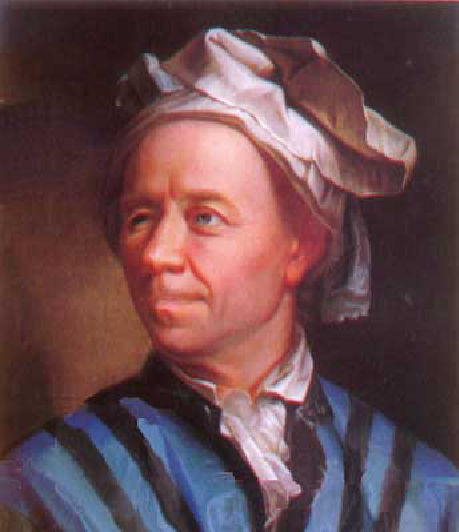
\includegraphics[width=\linewidth]{external/images/Euler.png}
			\end{image}%
			\tcblower
		\end{figureptx}%
		\footnotetext[10]{\nolinkurl{mathshistory.st-andrews.ac.uk/Biographies/Euler/}\label{g:fn:idp65}}%
		Leonhard Euler was a master at exploiting power series. In 1735, the 28 year-old Euler won acclaim for what is now called the Basel problem: to find a closed form for \(\sum_{n=1}^\infty\frac{1}{n^2}\). Other mathematicans knew that the series converged, but Euler was the first to find its exact value. The following problem essentially provides Euler's solution.%
		\begin{problem}{The Basel Problem.}{g:problem:idp66}%
			\begin{enumerate}[font=\bfseries,label=(\alph*),ref=\alph*]
				\item{}Show that the power series for \(\frac{\sin x}{x}\) is given by \(1-\frac{1}{3!}x^2+\frac{1}{5!}x^4-\cdots\)%
				\item{}Use (a) to infer that the roots of \(1-\frac{1}{3!}x^2+\frac{1}{5!}x^4-\cdots\) are given by%
				\begin{equation*}
					x=\pm\pi,\,\pm 2\pi,\,\pm 3\pi,\,\ldots
				\end{equation*}
				%
				\item{}Suppose \(p(x)=a_0+a_1x+\cdots+a_nx^n\) is a polynomial with roots \(r_1,\,r_2,\,\ldots,r_n\). Show that if \(a_0\neq\) \(0\), then all the roots are non-zero and%
				\begin{equation*}
					p(x)=a_0\left(1-\frac{x}{r_1}\right)\left(1-\frac{x}{r_2}\right)\cdots\left(1-\frac{x}{r_n}\right)\text{.}
				\end{equation*}
				%
				\item{}Assuming that the result in part (c) holds for an infinite polynomial (power series), deduce that%
				\begin{align*}
					1-\frac{1}{3!}x^2+\frac{1}{5!}x^4-\cdots\amp =\left(1-\left(\frac{x}{\pi}\right)^2\right)\left(1-\left(\frac{x}{2\pi}\right)^2\right)\left(1-\left(\frac{x}{3\pi}\right)^2\right)\cdots
				\end{align*}
				%
				\item{}Expand this product to deduce%
				\begin{equation*}
					\sum_{n=1}^\infty\frac{1}{n^2}=\frac{\pi^2}{6}.{}
				\end{equation*}
				%
			\end{enumerate}
		\end{problem}
		\begin{problem}{Euler's Formula.}{g:problem:idp67}%
			\begin{enumerate}[font=\bfseries,label=(\alph*),ref=\alph*]
				\item{}Use  the power series expansion of \(e^x\), \(\sin x,\) and \(\cos x\) to derive \terminology{Euler's Formula}:%
				\begin{equation*}
					e^{i\theta} = cos\theta+i\sin\theta.
				\end{equation*}
				%
				\item{}Use Euler's formula to derive the Addition\slash{}Subtraction formulas from Trigonometry:%
				\begin{equation*}
					\sin(\alpha\pm\beta) = \sin\alpha\cos\beta\pm\sin\beta\cos\alpha
				\end{equation*}
				%
				\begin{equation*}
					\cos(\alpha\pm\beta) = \cos\alpha\cos\beta\mp\sin\alpha\sin\beta
				\end{equation*}
				%
				\item{}Use Euler's formula to show that%
				\begin{equation*}
					\sin 2\theta = 2\cos\theta\sin\theta
				\end{equation*}
				%
				\begin{equation*}
					\cos 2\theta =\cos^2\theta-\sin^2\theta
				\end{equation*}
				%
				\item{}Use Euler's formula to show that%
				\begin{equation*}
					\sin 3\theta = 3\cos^2\theta\sin\theta-\sin^3\theta
				\end{equation*}
				%
				\begin{equation*}
					\cos 3\theta=\cos^3\theta-\cos\theta\sin^2\theta
				\end{equation*}
				%
				\item{}Find a formula \(\sin(n\theta)\) and \(\cos(n\theta)\) for any positive integer \(n\).%
			\end{enumerate}
		\end{problem}
	\end{sectionptx}
	%
	%
	\typeout{************************************************}
	\typeout{Section 4.3 Additional Problems}
	\typeout{************************************************}
	%
	\begin{sectionptx}{Additional Problems}{}{Additional Problems}{}{}{x:section:CalcIn17th18thCentury-AddProb}
		\begin{problem}{}{g:problem:idp68}%
			\index{series!Geometric series!alternating}\index{series!Geometric series!derivation of the series representation of \(\ln(1+x)\) from} Use the geometric series to obtain the series%
			\begin{align*}
				\ln \left(1+x\right)\amp =x-\frac{1}{2}x^2+\frac{1}{3}x^3-\cdots\\
				\amp =\sum_{n=0}^\infty\frac{(-1)^n}{n+1}x^{n+1}.{}
			\end{align*}
			%
		\end{problem}
		\begin{problem}{}{g:problem:idp69}%
			\index{power series!drills} \emph{Without} using Taylor's Theorem, represent the following functions as power series expanded about 0 (i.e., in the form \(\sum_{n=0}^\infty a_nx^n\)).%
			\begin{enumerate}[font=\bfseries,label=(\alph*),ref=\alph*]
				\item{}\(\ln\left(1-x^2\right)\)%
				\item{}\(\frac{x}{1+x^2}\)%
				\item{}\(\arctan \left(x^3\right)\)%
				\item{}\(\ln\left(2+x\right)\)%
				\par\smallskip%
				\noindent\textbf{\blocktitlefont Hint}.\hypertarget{g:hint:idp70}{}\quad{}\(2+x=2\left(1+\frac{x}{2}\right)\)%
			\end{enumerate}
		\end{problem}
		\begin{problem}{}{g:problem:idp71}%
			\index{power series!for \(a^x\) expanded about 0} Let \(a\) be a positive real number. Find a power series for \(a^x\) expanded about 0.%
			\par\smallskip%
			\noindent\textbf{\blocktitlefont Hint}.\hypertarget{g:hint:idp72}{}\quad{}\(a^x=e^{\ln\,\left(a^x\right)}\)%
		\end{problem}
		\begin{problem}{}{g:problem:idp73}%
			\index{power series!of \(\sin(x)\), expanded about \(a\)}\index{\(\sin x\)!as a power series} Represent the function \(\)sin \(x\) as a power series expanded about \(a\) (i.e., in the form \(\sum_{n=0}^\infty a_n\left(x-a\right)^n\)).%
			\par\smallskip%
			\noindent\textbf{\blocktitlefont Hint}.\hypertarget{g:hint:idp74}{}\quad{}\(\sin x=\sin \left(a+x-a\right)\).%
		\end{problem}
		\begin{problem}{}{g:problem:idp75}%
			\index{Maclaurin series drills} \emph{Without} using Taylor's Theorem, represent the following functions as a power series expanded about \(a\) for the given value of \(a\) (i.e., in the form \(\sum_{n=0}^\infty a_n\left(x-a\right)^n\)).%
			\begin{enumerate}[font=\bfseries,label=(\alph*),ref=\alph*]
				\item{}\(\ln x\), \(a=1\)%
				\item{}\(e^x\), \(a=3\)%
				\item{}\(x^3+2x^2+3\) , \(a=1\)%
				\item{}\(\frac{1}{x}\) , \(a=5\)%
			\end{enumerate}
		\end{problem}
		\begin{problem}{}{g:problem:idp76}%
			\index{series!term by term integration of} Evaluate the following integrals as series.%
			\begin{enumerate}[font=\bfseries,label=(\alph*),ref=\alph*]
				\item{}\(\displaystyle\int_{x=0}^1e^{x^2}\dx{ x}\)%
				\item{}\(\displaystyle\int_{x=0}^1\frac{1}{1+x^4}\dx{ x}\)%
				\item{}\(\displaystyle\int_{x=0}^1\sqrt[3]{1-x^3}\dx{ x}\)%
			\end{enumerate}
		\end{problem}
	\end{sectionptx}
\end{chapterptx}
%
%